\chapter{\tool{SysNut}: Um Sistema de Auxílio ao Nutricionista} \label{ch:sysnut}


{\color{red} Este capítulo apresenta o que é o \SysNut (Section \ref{sec:sysnut}), bem como \ldots, Feramentas utilizadas na contrução do sistema (Section \ref{sec:ferramental}), \ldots}  



\section{O que é o \SysNut?} \label{sec:sysnut}

\SysNut é um sistema Web que tem o propósito de apoiar as atividades do Nutriciionista. Mais especificamente, o sistema provê suporte para as seguintes atividades:

\begin{itemize}

\item auxilia nos cálculos da rotina de atendimento do paciente;
\item auxilia no agendamento de consultas;
\item {\color{red}tempo em que pudesse visualizar o progresso do paciente. Além disso, foi solicitado a possibilidade de adicionar cardápios as suas consultas para que o paciente possa seguir
suas recomendações.}

\end{itemize}
\ldots 



\section{Implementação das Rotinas do Nutricionista}

Durante todo o desenvolvimento, foi necessário conhecer e entender os
procedimentos de todas as partes (nutricionista e paciente), desde sua primeira visita
ao consultório até o acompanhamento do nutricionista com prescrição cardápio, para
que fosse possível atender às necessidades descritas para que os resultados
fossem mais claros e objetivos.

O sistema foi desenvolvido utilizando a metodologia Scrum (Seção 2.3.1), sem nenhum custo adicional
para os profissionais interessados, onde as análises são feitas sobre as histórias de usuário, sendo que cada uma delas
representa uma necessidade do usuário do sistema. Primeiramente, foi definido o
\textit{Product BackLog}, com as histórias de usuário relatadas pelo \textit{Product Owner}.

%Tabela 1
\begin{figure} [hbt] 
\begin{center}
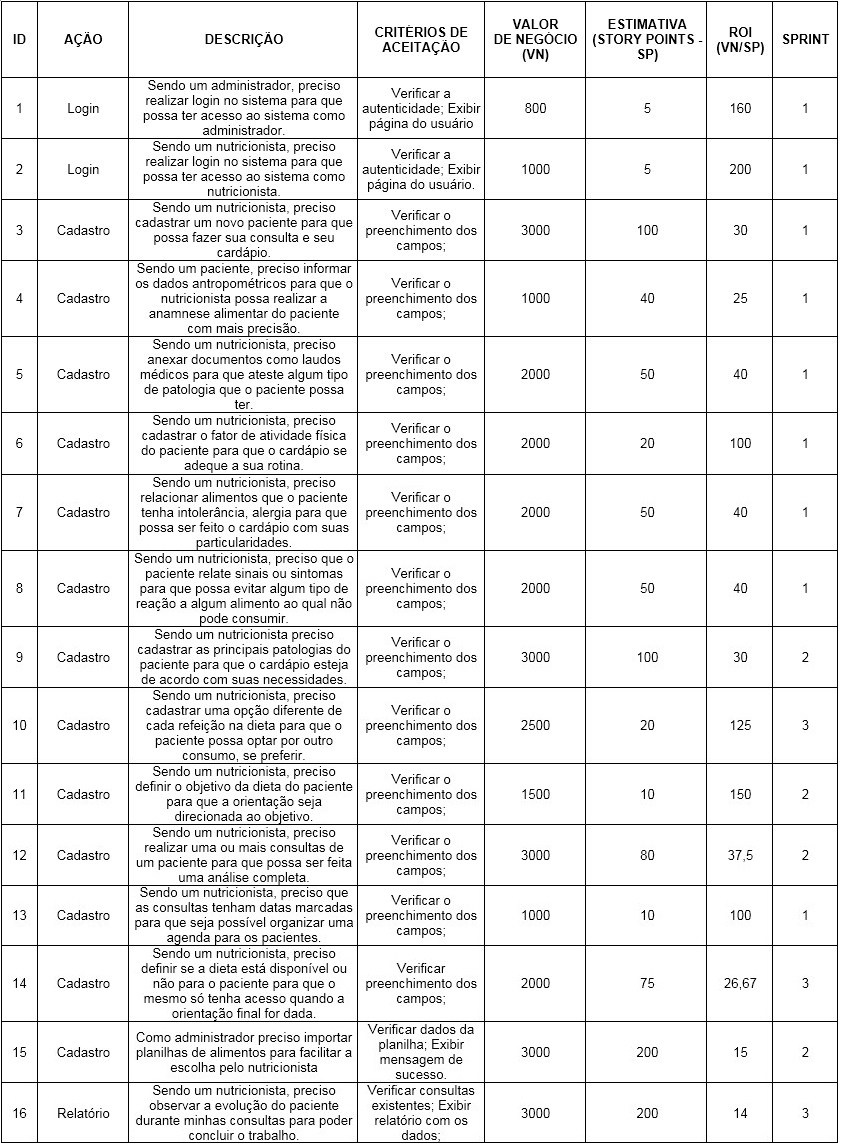
\includegraphics[width=0.90\textwidth]{table.jpg}
\end{center}
\label{table1} 
\caption{\textit{Product BackLog}}
\end{figure}

O \textit{Product BackLog} possui oito atributos, especificados na Figura 4: %colocar tabela

\begin{enumerate}

\item \textbf{ID}: identifica unicamente uma história do \textit{Product BackLog}.
\item \textbf{Ação}: define onde deve ser executado a história.
\item \textbf{Descrição}: contém a história de usuário
\item \textbf{Critérios de aceitação}: contém os critérios para que a ação possa ser
executada com êxito.
\item \textbf{Valor de Negócio}: define a importância da história.
\item \textbf{Estimativa (\textit{Story Points})}: estima o custo do (na visão do desenvolvedor)
para se implementar a história.
\item \textbf{ROI (VN/SP)}: retorno do investimento em relação ao custo.
\item \textbf{\textit{Sprint}}: define em que \textit{Sprint} a funcionalidade foi implementada.

\end{enumerate}

\section{Casos de Uso}

Com base nas histórias elencadas no \textit{Product BackLog}, o sistema foi divido em 2
subsistemas. O primeiro define as ações do administrador e do nutricionista. A Figura 5
mostra o diagrama de casos de uso.

\begin{figure} [hbt] 
\begin{center}
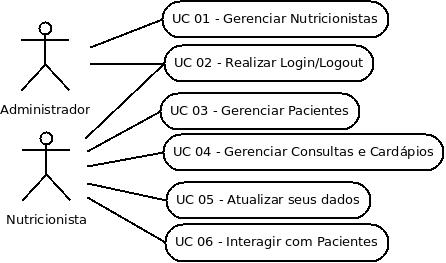
\includegraphics[width=0.9\textwidth]{uc1.jpeg}
\end{center}
\label{uc1} 
\caption{Casos de Uso Administrador e Nutricionista}
\end{figure}

\begin{itemize}
\item \textbf{UC01 – Gerenciar Nutricionistas}

\textbf{- Ator:} Administrador

\textbf{- Descrição:} O usuário administrador pode cadastrar, excluir e
editar os nutricionistas do sistema.

\item \textbf{UC02 – Realizar login e logout}

\textbf{- Ator:} Administrador e Nutricionista

\textbf{- Descrição:} Todos os usuários devem se autenticar, para que o
sistema os identifique e defina suas permissões de acesso.

\item \textbf{UC03 – Gerenciar Pacientes}

\textbf{- Ator:} Nutricionista

\textbf{- Descrição:} O nutricionista pode cadastrar, editar e excluir
pacientes do sistema.

\item \textbf{UC04 – Gerenciar Consultas/Cardápios}

\textbf{- Ator:} Nutricionista

\textbf{- Descrição:} O nutricionista pode cadastrar, editar e excluir
consultas e cardápios feitas sobre um paciente conforme acompanhamento.

\item \textbf{UC05 – Atualizar seus dados}

\textbf{- Ator:} Nutricionista

\textbf{- Descrição:} O nutricionista pode editar dados a seu respeito,
como Nome, E-mail, Senha de Login, etc.

\item \textbf{UC06 – Interagir com Pacientes}

\textbf{- Ator:} Nutricionista

\textbf{- Descrição:} O nutricionista poderá interagir com o paciente através de troca de mensagens pelo próprio sistema.

\end{itemize}

O segundo subsistema, deixa claro as ações do nutricionista em relação ao
paciente. A Figura 6 mostra o diagrama de casos de uso desse subsistema.

\begin{figure} [hbt] 
\begin{center}
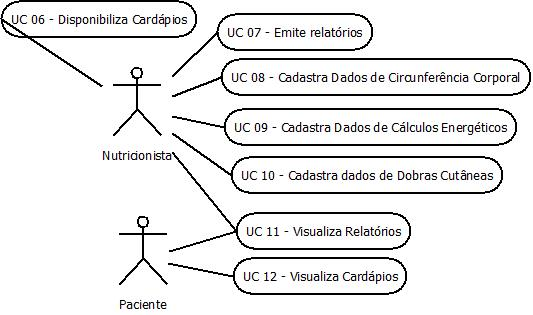
\includegraphics[width=1\textwidth]{uc2.jpeg}
\end{center}
\label{uc2} 
\caption{Casos de Uso Nutricionista e Paciente}
\end{figure}

O diagrama da Figura 6 visa deixar claro as principais ações do nutricionista
em relação ao paciente e o que o paciente pode fazer. Abaixo, segue a descrição
detalhada de cada caso de uso:

\begin{itemize}
\item \textbf{UC07 – Gerenciar Cardápio conforme feedback do paciente}

\textbf{- Ator:} Nutricionista

\textbf{- Descrição:} Uma vez que foi feita a consulta, o nutricionista poderá cadastrar cardápios e fazer alterações do mesmo conforme feedback do paciente.

\item \textbf{UC08 – Emitir relatórios}

\textbf{- Ator:} Nutricionista

\textbf{- Descrição:} O nutricionista é capaz de emitir e disponibilizar
relatórios ao paciente.

\item \textbf{UC09 – Cadastrar Dados de Circunferência Corporal, Cálculos Energéticos, Dobras Cutâneas, Diâmetro Ósseo e Bioimpedância}

\textbf{- Ator:} Nutricionista

\textbf{- Descrição:} O nutricionista poderá cadastrar dados de mensuração sobre o paciente durante a consulta e a partir deles acompanhar seu progresso.

\item \textbf{UC10 – Cadastrar dados de alergia, medicamentos e intolerâncias}

\textbf{- Ator:} Nutricionista

\textbf{- Descrição:} O nutricionista poderá salvar dados acerca de patologias que o paciente possui e medicamentos que ele usa ou possa vir a usar.

\item \textbf{UC11 – Acompanhar o Paciente através de troca de mensagens}

\textbf{- Ator:} Nutricionista

\textbf{- Descrição:} O nutricionista poderá acompanhar o progresso do paciente através de troca de mensagens e por meio delas receber \textit{feedback}.

\item \textbf{UC12 – Visualizar Relatórios e Cardápios}

\textbf{- Atores:} Nutricionista e Paciente

\textbf{- Descrição:} O nutricionista e seu paciente poderão visualizar cardápios e relatórios assim que forem salvos pelo próprio nutricionista.

\item \textbf{UC13 – Interagir com o Nutricionista}

\textbf{- Atores:} Paciente

\textbf{- Descrição:} O paciente poderá interagir com o nutricionista por meio de mensagens e através delas sugerir alterações no cardápio.

\item \textbf{UC14 – Atualizar seus dados}

\textbf{- Atores:} Paciente

\textbf{- Descrição:} O paciente poderá alterar seus próprios dados como login e senha, nome e sobrenome, entre outros.

\end{itemize}

A Figura 7, relaciona as classes do sistema e seus respectivos campos.

\begin{figure} [hbt] 
\begin{center}
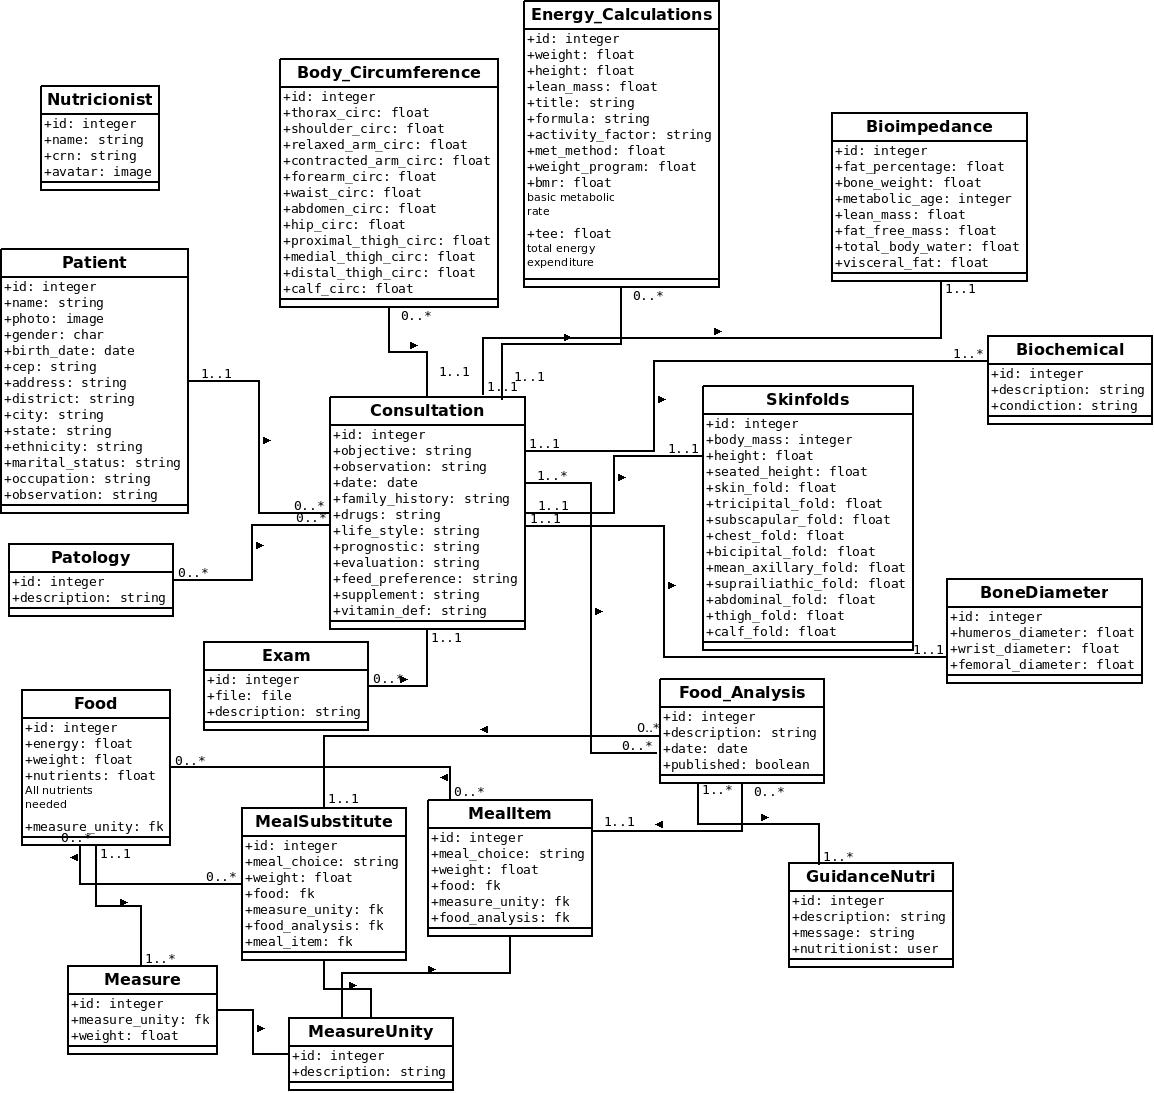
\includegraphics[width=1\textwidth]{bd-sistema.jpeg}
\end{center}
\label{diagClass1} 
\caption{Diagrama de Classes do Sistema}
\end{figure}

O nutricionista é quem cadastra novos pacientes. O paciente possui dados como
dobras cutâneas, circunferência corporal e dados para cálculos energéticos. O
paciente também pode possuir patologias, onde estas podem interferir na sua
alimentação. Além disso, poderá ser cadastrado exames feitos sobre um paciente e
orientações sobre um determinado cardápio. 

Dados como etnia, profissão podem influenciar no fator de atividade física e portanto,
enfatiza-se a presença destes no diagrama da Figura 7. É possível cadastrar cada um destes
dados durante a consulta do paciente. Após feita a consulta, o nutricionista poderá
cadastrar cardápios e consequentemente os alimentos a serem consumidos em cada refeição.
Durante o cadastro de um novo cardápio, o nutricionista seleciona o alimento,
o horário em que será consumido, a quantidade normal, a medida caseira e se este
será publicado ou não, podendo ser editado posteriormente.

Cada alimento, possui micro e macro nutrientes como energia, carboidratos,
lipídios, entre outros. Estes devem ser previamente cadastrados antes de prescrever o
cardápio.

\section{Telas do sistema}

Nesta seção, são apresentadas telas, obtidas durante a implementação do sistema.

\begin{figure} [hbt] 
\begin{center}
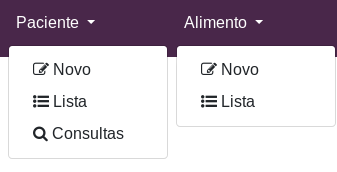
\includegraphics[width=0.55\textwidth]{menuNut1.png}
\end{center}
\label{menuNut} 
\caption{Menu do Nutricionista}
\end{figure}

\begin{figure} [hbt] 
\begin{center}
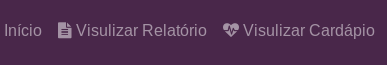
\includegraphics[width=0.55\textwidth]{menuPac1.png}
\end{center}
\label{menuPac} 
\caption{Menu do Paciente}
\end{figure}

É possível observar nas Figuras 8 e 9 que ambos (paciente e nutricionista) podem ter acesso as suas funcionalidades que ficam localizadas na barra superior do navegador.
A Figura 8 mostra todas as funcionalidades do Nutricionista. O Nutricionista
ainda pode emitir relatórios a partir da lista de pacientes acessível no menu. Cada
funcionalidade dessa fica disponível a partir do momento que o Nutricionista realiza 
Login no sistema. A Figura 9 mostra o menu do Paciente. O paciente pode obter dados
do relatório ou do cardápio apenas digitando seu ID e senha do sistema.
Como já mencionado anteriormente, o \textit{Django} possui um sistema de URL's e é através dele que
é feito o tratamento de permissões, uma vez que somente o nutricionista é autorizado de fazer cadastro
de pacientes. A Figura 10 mostra um exemplo de lista de usuários previamente cadastrados no sistema.

\begin{figure} [hbt]
\begin{center}
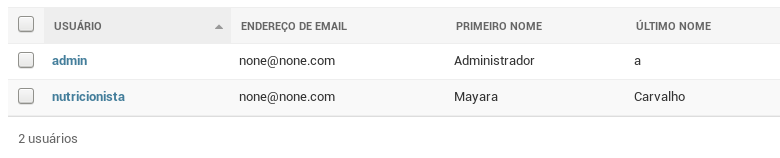
\includegraphics[width=0.55\textwidth]{listaUsuarios.png}
\end{center}
\label{listUser} 
\caption{Lista de Usuários Cadastrados}
\end{figure}

A Figura 11 mostra a tela de cadastro de pacientes, onde é possível cadastrar
seus dados pessoais e os demais dados para fins de acompanhamento do paciente. 

\begin{figure} [hbt]
\begin{center}
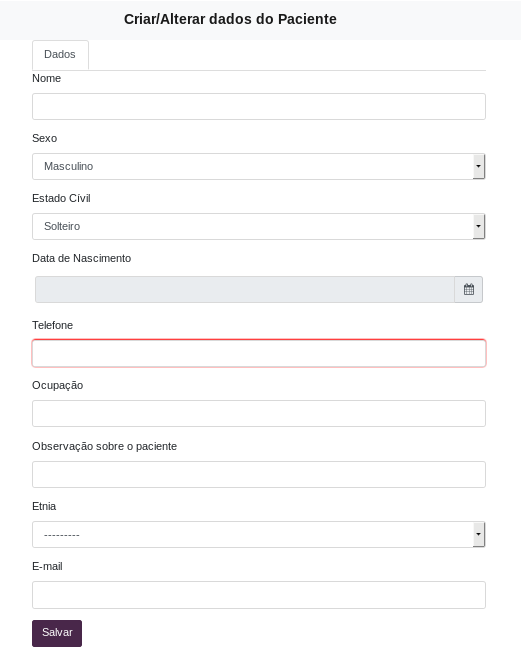
\includegraphics[width=0.55\textwidth]{cadastroPac1.png}
\end{center}
\label{cadastroPac} 
\caption{Tela de Cadastro de Pacientes}
\end{figure}

\begin{figure} [hbt]
\begin{center}
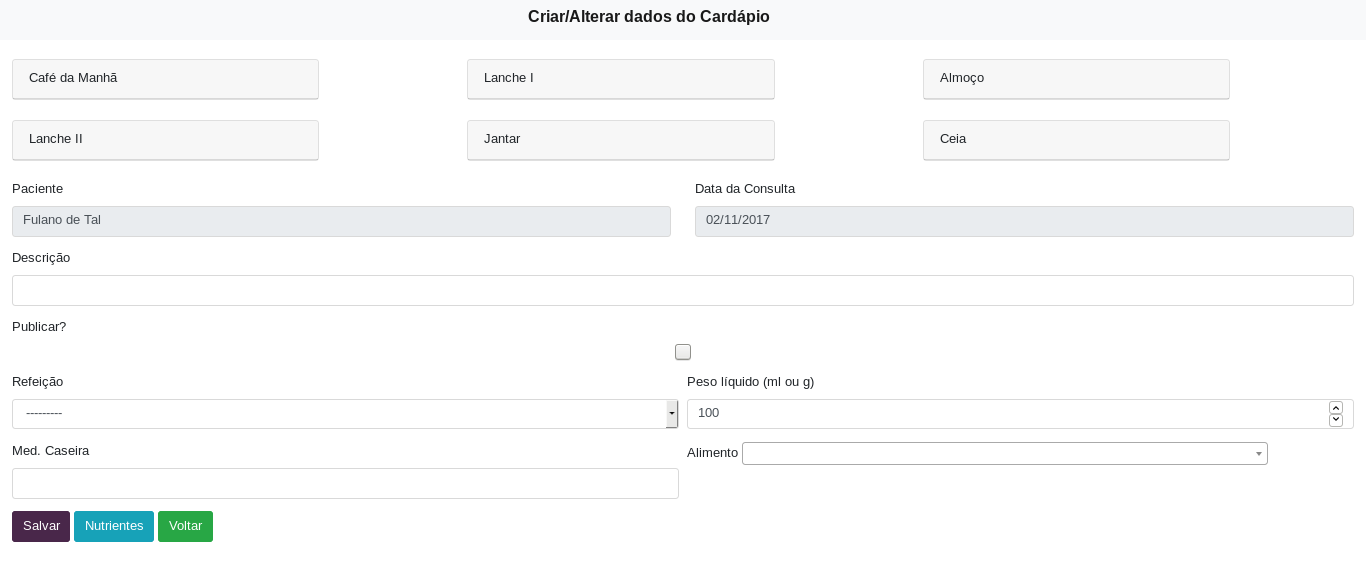
\includegraphics[width=0.55\textwidth]{cadastroCard.png}
\end{center}
\label{cadastroCard} 
\caption{Tela de Cadastro de Cardápio}
\end{figure}

\begin{figure} [hbt]
\begin{center}
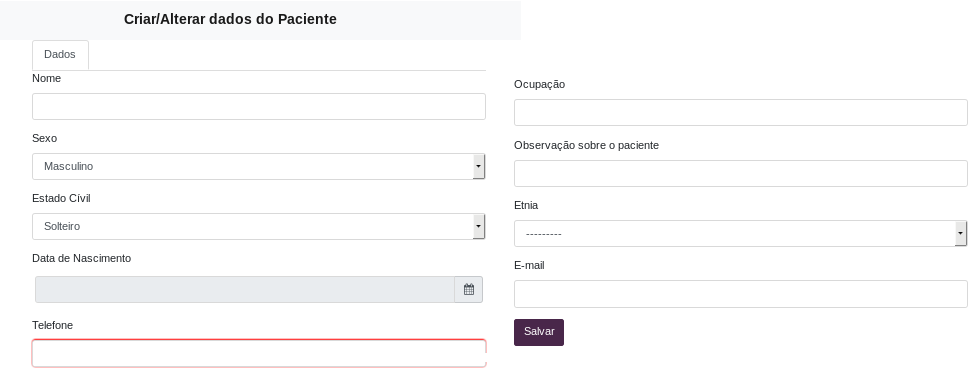
\includegraphics[width=0.55\textwidth]{cadastroCons1.png}
\end{center}
\label{cadastroCons} 
\caption{Tela de Cadastro de Consulta}
\end{figure}

As Figuras 12 e 13 mostram as telas de cadastro de cardápio e consulta,
respectivamente. É durante a consulta que o nutricionista cadastra os dados de
acompanhamento do paciente. O cardápio só poderá ser cadastrado se a consulta já
tiver sido cadastrada previamente.

No cadastro de consultas, o nutricionista cadastra informações de histórico
familiar do paciente, patologias, fármacos que utiliza, além de dados de
acompanhamento como dobras cutâneas, circunferência corporal, entre outros.

O cadastro de cardápio consta dados do paciente, como nome completo e data
em que a consulta foi realizada. Em seguida, a descrição do cardápio, disponibilidade
e os alimentos a serem cadastrados, que devem ter horário de consumo, quantidade
e medida caseira.

\begin{figure} [hbt]
\label{relatPac} 
\caption{Relatório do Paciente}
\begin{center}
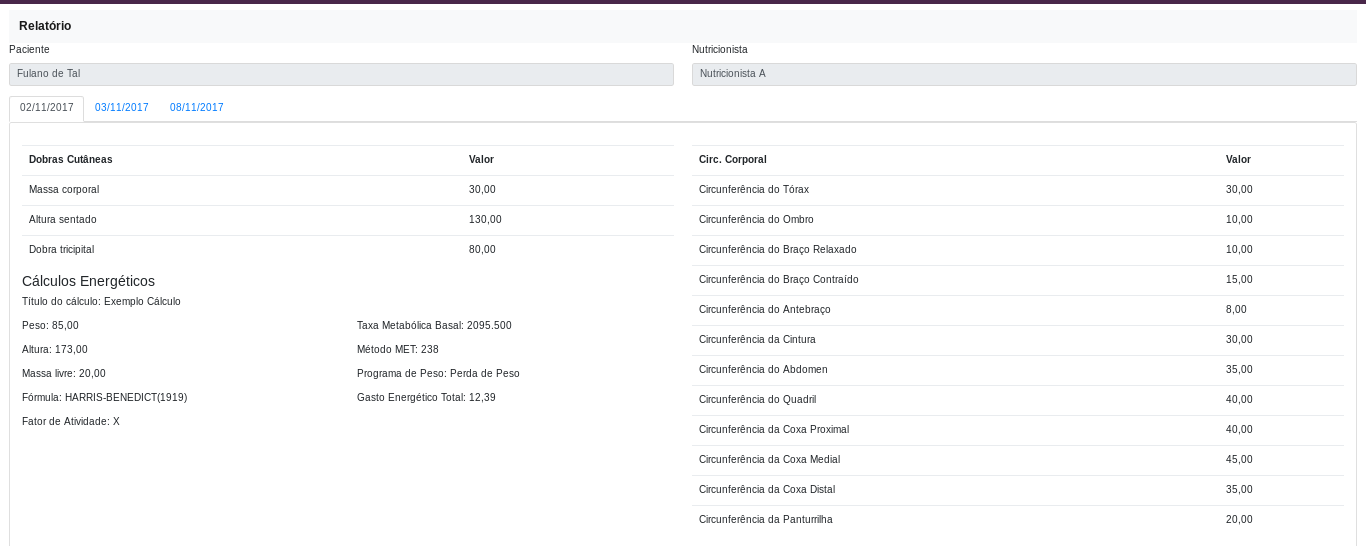
\includegraphics[width=0.75\textwidth]{relatPac1.png}
\end{center}
\end{figure}

A Figura 14 mostra o relatório do paciente, onde é possível ver todos os dados
durante as consultas que foram realizadas e os dados de acompanhamento que foram
obtidos em cada uma delas.

A Figura 15 mostra o cardápio com a descrição e todas as suas informações
nutricionais (macro e micro nutrientes), além do nome do paciente para quem foi
prescrito.
Todas as funcionalidades aqui apresentadas, atualmente, encontram-se
implementadas e já estão prontas para serem usufruidas pelos profissionais interessados.

\begin{figure} [hbt]
\begin{center}
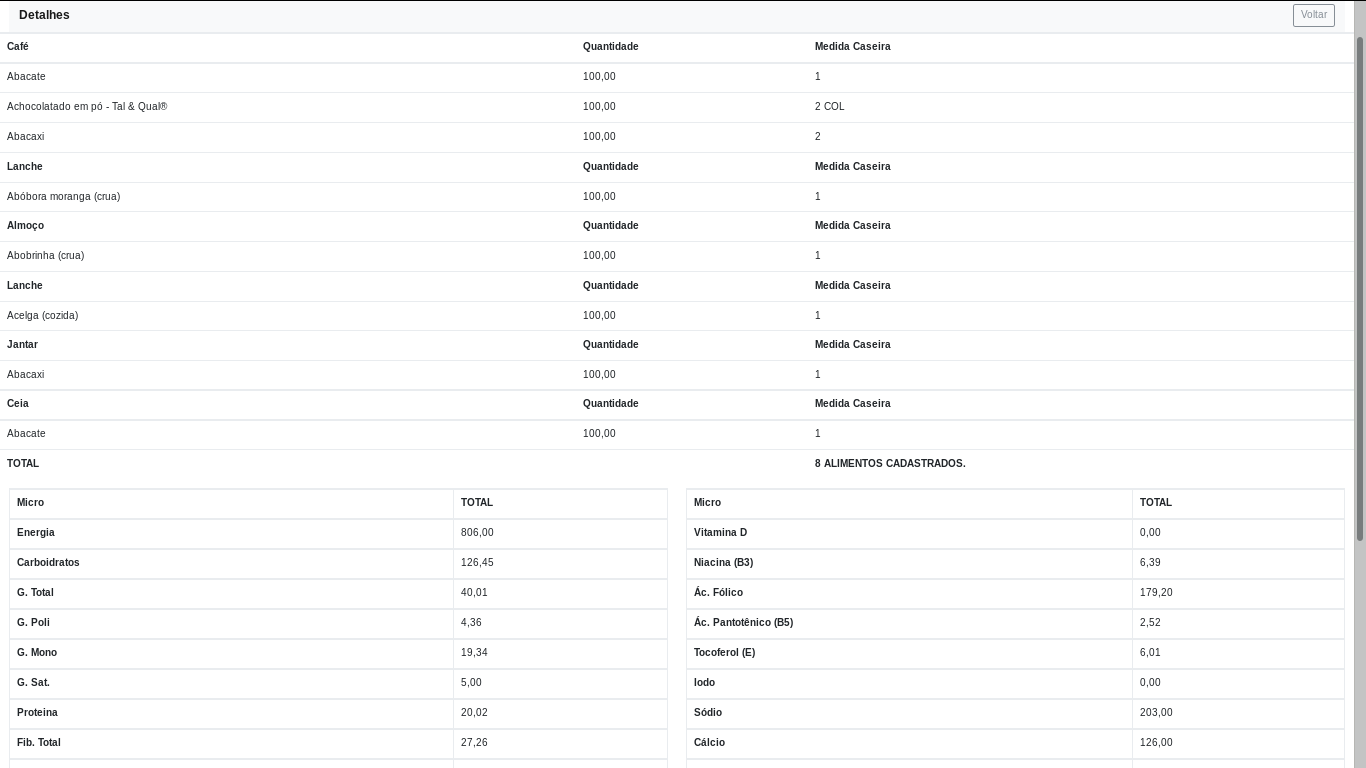
\includegraphics[width=1.0\textwidth]{cardPac1.png}
\end{center}
\label{cardPac} 
\caption{Cardápio do Paciente}
\end{figure}


\section{Ferramentas Utilizadas} \label{sec:ferramental}

Esta seção apresenta os conceitos utilizados durante o desenvolvimento do projeto. \citeonline{tenorio} ressalta a importância da organização e compreensão das informações de um sistema \textit{Web} por parte do usuário, atendendo às necessidades e exigências do mesmo durante o desenvolvimento do sistema.


% --- Seção dentro do capítulo
\subsection{Desenvolvimento \textit{Backend}}
% ---

O lado servidor é onde deve funcionar a lógica principal da aplicação. Todas as
ações são tratadas como requisição. Quando o usuário faz a requisição ao servidor,
é chamado de HTTP \textit{request}. Quando a resposta é enviada pelo servidor, esta ação
é chamada de HTTP \textit{response}.

Os sistemas \textit{Web} funcionam da seguinte maneira: o usuário (cliente) faz uma
requisição de uma página para o servidor e retorna uma resposta para ele através do
navegador. A resposta é interpretada pelo navegador e entregue pelo servidor para o
usuário \cite{niederauer}.

\subsubsection{Python}

Python é uma linguagem de programação de altíssimo nível, orientada a objeto
e de tipagem dinâmica e forte, interpretada e interativa. O nome Python foi dado por
Guido van Rossum do programa da TV Britânica \textit{Monty Python’s Flying Circus} e a
linguagem foi criada por ele, na década de 90, no Instituto Nacional de Pesquisa para
Matemática e Ciência da Computação da Holanda (CWI). O Python foi concebido a
partir de outra linguagem existente na época, chamada ABC.

A intenção do autor ao criar a linguagem é que fosse de altíssimo nível e que
tivesse características importantes de outras linguagens de programação. Python é
livre, ou seja, tem código aberto, com licença compatível com a \textit{General Public License}
(GPL). A especificação da linguagem é mantida pela \textit{\textit{Python Software Foundation}}
(PSF). A linguagem Python apresenta uma série de vantagens e recursos
interessantes que foram inspirados e aproveitados de outras linguagens de sucesso,
tornando-a assim uma linguagem bastante flexível \cite{borges}.

Python possui diversas características e estruturas de alto nível (listas,
dicionários, entre outros) e uma coleção de módulos prontos para uso, além de outras
ferramentas que podem ser utilizadas para auxiliar no desenvolvimento, dentre elas
citamos o Django, que será abordado no tópico a seguir.

Segundo \citeonline{diakopoulos}, Python lidera o ranking de linguagens
mais utilizadas, seguido por C e Java. Existem também implementações de Python
para .NET (IronPython), JVM (Jython), entre outros.

\subsubsection{Django}

O Django é um \textit{framework} de desenvolvimento \textit{Web} criado por Jacob Kaplan Moss,
Adrian Holovaty e Simon Willison em 2003. O Django utiliza o conceito DRY –
\textit{Don’t Repeat yourself} (“não repita a si mesmo”), que propõe que cada parte de um
sistema deve possuir uma representação única.

O Django possui vários componentes com funções específicas. \citeonline{neto}
cita alguns de seus principais componentes:

 \begin{itemize}

	\item \textbf{ORM} (\textit{Object-relational mapper} - Mapeador objeto-relacional): é
uma técnica de mapeamento objeto relacional que permite fazer uma
relação dos objetos com os dados que estes representam.
	\item \textbf{\textit{Template System}}: linguagem para criação de templates (HTML, XML,
JSON, etc.) usados na geração de páginas dinâmicas.
Sistema de administração: Interface de administração própria do
\textit{framework} (Django-admin).
	\item \textbf{URL} (\textit{Uniform Resource Locator}) \textit{dispatcher}: Processador de URLs
do sistema que executando funções específicas feitas pelo
desenvolvedor, possibilitando URL’s amigáveis.
	\item \textbf{Internacionalização}: permite que o sistema seja traduzido para
diversos idiomas.
	\item \textbf{Formulários}: geração automática de formulários e facilitação na
manipulação dos dados enviados por meio deles.
	\item \textbf{Segurança}: gerenciamento de autenticação de usuários e controle de
permissões.
	\item \textbf{Outros componentes}: serialização de dados, sistema de testes
automatizado, entre outros.

\end{itemize}

O padrão de projeto MVC (\textit{Model-View-Controller}) divide-se em três camadas: Modelo, Visão e
Controlador. O Modelo é o responsável pela comunicação com os dados
armazenados no banco de dados que serão visualizados na camada de Visão. A
Visão, por sua vez, é responsável pela apresentação da aplicação. E por último, o
controlador, responsável por administrar todo o fluxo da aplicação \cite{lemos}.

O Django utiliza o padrão de projeto MTV (\textit{Model-Template-View}) para
desenvolvimento, que possui essencialmente a mesma lógica que o MVC,
muito utilizado em outras linguagens \cite{neto}. A diferença é apenas conceitual. A camada \textit{Template}
executa exatamente a mesma função que a camada \textit{View} do MVC, o mesmo vale para a camada \textit{View} em
relação a camada \textit{Controller} do MVC, com uma ressalva de que os desenvolvedores do \textit{framework} entendem
que o controlador é a própria ferramenta \cite{django}.

\subsubsection{Banco de Dados MySQL}
O MySQL, criado pela empresa MySQL AB na Suécia, é um SGBD que utiliza a
linguagem SQL como interface. A MySQL AB foi adquirida pela Sun Microsystems em
2008, a qual posteriormente foi comprada pela Oracle, incluindo o SGBD MySQL.
Atualmente, esse é um dos bancos de dados mais utilizados do mundo, com mais de
10 milhões de instalações e um dos motivos para essa popularidade é devido a fácil
integração a também popular linguagem PHP \cite{mottin}. Entre os usuários mais populares do MySQL estão: NASA, Bradesco, Dataprev, HP, Nokia, Sony, Sistemas Cisco, entre outros.
O MySQL é o banco de dados de código aberto mais popular do mundo. Ainda
mantido pela Oracle, tornou-se a principal escolha de banco de dados para aplicativos
\textit{Web}, usado por \textit{websites} muito conhecidos como: Facebook, Twitter, YouTube, entre
outros.

Dentre as características do MySQL, é possível citar: portátil (suporta qualquer plataforma), compatível (possui compatibilidade com diversas linguagens de programação), é um software livre (licença GPL), pouco exigente quanto ao hardware e é fácil de utilizar.

% --- Seção dentro do capítulo
\subsection{Desenvolvimento \textit{Frontend}}
% ---

O lado cliente de uma aplicação \textit{Web} é quem realiza a requisição e se comunica
com o servidor, ao tempo que recebe a resposta do mesmo. Em outras palavras, o
lado cliente é quem estabelece a comunicação com o usuário.

\subsubsection{HTML}

HTML é uma sigla em inglês que significa Linguagem para Marcação de
Hipertexto (\textit{HyperText Markup Language}). Na aplicação, é usada para denotar os 
elementos da página, tais como caixas de seleção, caixas de texto, entre outros. Sua função é
definir apenas a estrutura da página \cite{folle}. A Figura 1 é um exemplo simples de uma página com código HTML, mostrando
algumas tags HTML e suas funcionalidades de marcação:
\begin{itemize}

	\item Tag <html> - delimita o início e o fim de uma página HTML. Tudo que pertence a página deve estar dentro dessa tag.
	\item Tag <head> - contém informações de cabeçalho da página, como: título,
	\item Tag <title> - define o título da página.
	\item Tag <body> - delimita o conteúdo que estará no corpo da página.

\end{itemize}

\begin{figure} [hbt] 
%% hbt SIGNIFICA QUE ELE PRIMEIRO VAI TENTAR COLOCAR A IMAGEM NESTE LUGAR (h de "here"). SENÃO DER, ELE TENTA COLOCAR MAIS PRA BAIXO (b de "bottom"). SENÃO ELE COLOCA MAIS PARA CIMA (t de "top").
\begin{center}
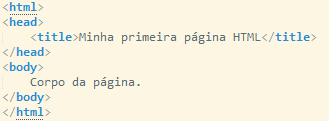
\includegraphics[width=0.75\textwidth]{exhtml.png} %% PARA COLOCAR O ARQUIVO DA IMAGEM NO SHARELATEX, CLIQUE NO ÍCONE QUE PARECE UMA FLECHINHA PARA CIMA (ATUALIZAR), CLIQUE EM UPLOAD E PROCURE A IMAGEM EM SEU COMPUTADOR.
\end{center}
\label{figura1} 
%% LABEL SERVE PARA VOCÊ REFERENCIAR A FIGURA NO MEIO DO TEXTO (VEJA LINHA 330: \ref{figura1}). ASSIM VOCÊ NÃO PERDE A REFERÊNCIA QUANDO MUDA A FIGURA DE LUGAR
\caption{Exemplo de código HTML.}
\end{figure}

\subsubsection{\textit{Cascading Style Sheets} – CSS}

CSS (\textit{Cascading Style Sheets}) – é uma linguagem utilizada para tratamento
visual dos elementos da página \textit{Web} \cite{folle}. Este é, portanto, a tecnologia
responsável por tratar cada elemento da página \textit{Web} visualmente, atribuindo cores e
posições diferentes, dependendo da preferência do programador. Possui sintaxe
simples e assim como as demais tecnologias, utiliza-se de várias palavras em inglês
para especificar os diferentes estilos de propriedades da página.

\begin{figure} [hbt] 
\begin{center}
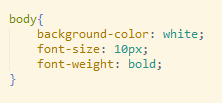
\includegraphics[width=0.75\textwidth]{excss.png}
\end{center}
\label{figura1} 
\caption{Exemplo de código CSS.}
\end{figure}

\subsubsection{\textit{JavaScript e JQuery}}

Segundo \citeonline{folle}, \textit{JavaScript} “é uma linguagem de script executada pelos
navegadores que permite o acesso e manipulação programática de objetos de uma
página \textit{Web}”. Ela possibilita que um campo para digitar uma data seja formatado
automaticamente (com barras), ou que um campo seja desabilitado dinamicamente,
etc. 

\textit{JQuery} é portanto, uma biblioteca de funções prontas de \textit{JavaScript}, que
interagem com o HTML e possibilitam uma melhor experiência ao usuário. Foi lançada
em 2006, no BarCamp, de Nova York, por John Resig e é utilizada por milhares de
sites visitados pelo mundo. Segundo a \citeonline{w3techs}, é a biblioteca JavaScript
mais popular dentre as existentes



\subsection{\textit{Bootstrap}}

\textit{Bootstrap} é o mais popular \textit{framework} de HTML, CSS e \textit{JavaScript} para desenvolvimento de sistemas \textit{Web} de modo responsivo. Esta ferramenta conta com centenas de classes HTML que auxiliam na construção de uma página \textit{Web} \cite{bootstrap}.
Esta ferramenta está presente em cada página do sistema, possibilitando que ele seja acessado de qualquer dispositivo (móvel ou \textit{desktop}). A sua versão estável é a 3.3.7, mas já foi disponibilizada oficialmente a versão 4, versão esta utilizada neste projeto.



\section{Licensa do Software}

O software estará disponível em \url{...} sob a lincensa ???s